\documentclass{standalone}
\usepackage[T1]{fontenc}
\usepackage[latin2]{inputenc}
\usepackage[english]{babel}
\usepackage{tikz}
\usepackage{times}
\usetikzlibrary{calc,through,backgrounds,positioning,fit}
\usetikzlibrary{shapes,arrows,shadows}
 
\begin{document}
 
\begin{tikzpicture}

\node (rys1) at (0,0){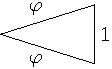
\includegraphics{rysunek1.pdf}};
\node (rys2) at (6,0){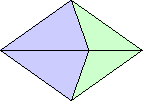
\includegraphics{rysunek2.pdf}};
\node (rys3) at (0,-3){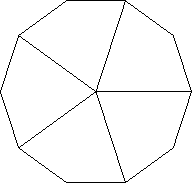
\includegraphics{rysunek3.pdf}};
\node (rys4) at (6,-3){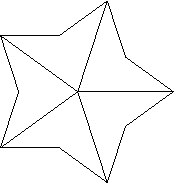
\includegraphics{rysunek4.pdf}};

\end{tikzpicture}
 
\end{document}